%%%%%%%%%%%%%%%%%%%%%%%%%%%%%%%%%%%%%%%%%%%%%%%%%%%%%%%%%%%%%%%%%%
%%%%%%%%%%%%%%%%%%%%%%%%%%%%%%%%%%%%%%%%%%%%%%%%%%%%%%%%%%%%%%%%%%
%Packages
\documentclass[10pt, a4paper]{article}
\usepackage[top=3cm, bottom=4cm, left=3.5cm, right=3.5cm]{geometry}
\usepackage{amsmath,amsthm,amsfonts,amssymb,amscd, fancyhdr, color, comment, graphicx, environ}
\usepackage{float}
\usepackage{mathrsfs}
% \setmathfont{TeX Gyre Termes Math}
\usepackage{lastpage}
\usepackage[dvipsnames]{xcolor}
\usepackage[framemethod=TikZ]{mdframed}
\usepackage{enumerate}
\usepackage[shortlabels]{enumitem}
\usepackage{fancyhdr}
\usepackage{indentfirst}
\usepackage{listings}
\usepackage{sectsty}
\usepackage{thmtools}
\usepackage{shadethm}
\usepackage{hyperref}
\usepackage{setspace}
\usepackage{changepage}
\usepackage[linguistics]{forest}
\usepackage[english]{babel}
\usepackage{blindtext}
\RequirePackage{filecontents}
\hypersetup{
    colorlinks=true,
    linkcolor=blue,
    filecolor=magenta,
    urlcolor=blue,
}
\mdfsetup{skipabove=\topskip,skipbelow=\topskip}
\newrobustcmd\ExampleText{%
An \textit{inhomogeneous linear} differential equation has the form
\begin{align}
L[v ] = f,
\end{align}
where $L$ is a linear differential operator, $v$ is the dependent
variable and $f$ is a given non−zero function of the independent
variables alone.
}
\mdfdefinestyle{theoremstyle}{%
linecolor=black,linewidth=1pt,%
frametitlerule=true,%
frametitlebackgroundcolor=gray!20,
innertopmargin=\topskip,
}
\mdtheorem[style=theoremstyle]{Problem}{Problem}
\newenvironment{Solution}{\textbf{Solution.}}

\definecolor{codegreen}{rgb}{0,0.6,0}
\definecolor{codegray}{rgb}{0.5,0.5,0.5}
\definecolor{codepurple}{rgb}{0.58,0,0.82}
\definecolor{backcolour}{rgb}{0.95,0.95,0.92}

\lstdefinestyle{mystyle}{
    backgroundcolor=\color{backcolour},   
    commentstyle=\color{codegreen},
    keywordstyle=\color{magenta},
    numberstyle=\tiny\color{codegray},
    stringstyle=\color{codepurple},
    basicstyle=\ttfamily\footnotesize,
    breakatwhitespace=false,         
    breaklines=true,                 
    captionpos=b,                    
    keepspaces=true,                 
    numbers=left,                    
    numbersep=5pt,                  
    showspaces=false,                
    showstringspaces=false,
    showtabs=false,                  
    tabsize=2
}

\lstset{style=mystyle}
%%%%%%%%%%%%%%%%%%%%%%%%%%%%%%%%%%%%%%%%%%%%%%%%%%%%%%%%%%%%%%%%%%
%%%%%%%%%%%%%%%%%%%%%%%%%%%%%%%%%%%%%%%%%%%%%%%%%%%%%%%%%%%%%%%%%%
%Fill in the appropriate information below
\newcommand{\norm}[1]{\left\lVert#1\right\rVert}     
\newcommand\course{Course}                            % <-- course name   
\newcommand\hwnumber{Phys 338}                                 % <-- homework number
\newcommand\Information{Khaled Hasan}                        % <-- personal information
%%%%%%%%%%%%%%%%%%%%%%%%%%%%%%%%%%%%%%%%%%%%%%%%%%%%%%%%%%%%%%%%%%
%%%%%%%%%%%%%%%%%%%%%%%%%%%%%%%%%%%%%%%%%%%%%%%%%%%%%%%%%%%%%%%%%%
%Page setup
\pagestyle{fancy}
\headheight 35pt
\lhead{\today}
\rhead{
\includegraphics[width=2.5cm]{bzu-footer-logo.png}}
\lfoot{}
\pagenumbering{arabic}
\cfoot{\small\thepage}
\rfoot{}
\headsep 1.2em
\renewcommand{\baselinestretch}{1.25}
%%%%%%%%%%%%%%%%%%%%%%%%%%%%%%%%%%%%%%%%%%%%%%%%%%%%%%%%%%%%%%%%%%
%%%%%%%%%%%%%%%%%%%%%%%%%%%%%%%%%%%%%%%%%%%%%%%%%%%%%%%%%%%%%%%%%%
%Add new commands here
\renewcommand{\labelenumi}{\alph{enumi})}
\newcommand{\Z}{\mathbb Z}
\newcommand{\R}{\mathbb R}
\newcommand{\Q}{\mathbb Q}
\newcommand{\NN}{\mathbb N}
\newcommand{\PP}{\mathbb P}
\DeclareMathOperator{\Mod}{Mod} 
\renewcommand\lstlistingname{Algorithm}
\renewcommand\lstlistlistingname{Algorithms}
\def\lstlistingautorefname{Alg.}
\newtheorem*{theorem}{Theorem}
\newtheorem*{lemma}{Lemma}
\newtheorem{case}{Case}
\newcommand{\assign}{:=}
\newcommand{\infixiff}{\text{ iff }}
\newcommand{\nobracket}{}
\newcommand{\backassign}{=:}
\newcommand{\tmmathbf}[1]{\ensuremath{\boldsymbol{#1}}}
\newcommand{\tmop}[1]{\ensuremath{\operatorname{#1}}}
\newcommand{\tmtextbf}[1]{\text{{\bfseries{#1}}}}
\newcommand{\tmtextit}[1]{\text{{\itshape{#1}}}}

\newenvironment{itemizedot}{\begin{itemize} \renewcommand{\labelitemi}{$\bullet$}\renewcommand{\labelitemii}{$\bullet$}\renewcommand{\labelitemiii}{$\bullet$}\renewcommand{\labelitemiv}{$\bullet$}}{\end{itemize}}
\catcode`\<=\active \def<{
\fontencoding{T1}\selectfont\symbol{60}\fontencoding{\encodingdefault}}
\catcode`\>=\active \def>{
\fontencoding{T1}\selectfont\symbol{62}\fontencoding{\encodingdefault}}
\catcode`\<=\active \def<{
\fontencoding{T1}\selectfont\symbol{60}\fontencoding{\encodingdefault}}

\begin{document}

\begin{titlepage}
    \begin{center}
        \vspace*{3cm}
            
        \Huge
        \textbf{Wavefunction of an electron in an arbitrary Potential}
            
        \vspace{1cm}
        \huge
        Phys 338: Indevisual Project Report
            
        \vspace{1.5cm}
        \Large
            
        \textbf{Khaled Hasan 1210265}                      % <-- author
        
            
        \vfill
        
        \course: Computational Physics
            
        \vspace{1cm}
        
        \Large
        
        \today
            
    \end{center}
\end{titlepage}
\begin{filecontents}{mybib.bib}
@misc{cite1,
  title = {Drag Coefficient},
  howpublished = {\url{https://en.wikipedia.org/wiki/Drag_coefficient}},
  note = {Accessed: 2010-09-30}
}
\end{filecontents}
%Start the assignment now %%%%%%%%%%%%%%%%%%%%%%%%%%%%%%%%%%%%%%%%%%%%%%%%%%%%%%%%%%%%%%%%%%
%New problem
\newpage
\tableofcontents
\newpage
\section{{\Large Abstract}}
    \begin{adjustwidth}{1cm}{}
    The wave function is a complex function that describes the probability density of the existence of an electron in certain position in space (that is upon taking the norm squared of it), this suggests a dual behaviour of an electron, and that it acts as a wave.\\
    The dual behaviour of electrons that was proposed by de Broglie, using the Schrodinger equation which describes the wave function of an electron in a potential energy given by the potential operator $V(x, y, z)$. As the potential changes, the solution of the wave function changes, and due to the complexity of the partial differential equations, wave functions tends to get more and more complicated, even for simple potentials such as the harmonic oscillator. The solution is hard to treat analytically, and can only be solved using special functions ("Hermite Polynomials").\\
    This Problem of having complicated solutions that are easily effected by the small changes in potential, encourages the use of computational methods, in order to solve for the wave function of the electron.\\
    In this project, the Schrodinger equation was solved in one and two dimensions, for arbitrary potential.\\
    \end{adjustwidth}


    \section{{\Large Theory}}
    \begin{adjustwidth}{1cm}{}
    The Schrodinger Equation
    \begin{equation}    
    i\hbar\frac{\partial_x \vert\psi \left(x, y, z ,t\right)\rangle}{\partial t} = \hat{H}\vert\psi\left(x, y, z, t\right)\rangle
    \end{equation}

    Where $H$ is the hameltonian defined as:
    \begin{equation}\label{eq2}
        \hat{H} = \frac{-\hbar^2}{2m}\nabla^2 + V\left(x, y, z\right)
    \end{equation}
    from here on, the position parameters are dropped.\\
    The Taylor expansion of $\vert \psi(t) \rangle$
    \begin{equation}
        \vert\psi(t)\rangle = \vert\psi(0)\rangle + t\frac{\partial\vert\psi(t)\rangle}{\partial t}|t=0 +\frac{t^2}{2!}\frac{\partial^2\vert\psi(t)\rangle}{\partial t^2} |t=0 + ...
    \end{equation}
    substituting from equation \ref{eq2}:
    \begin{equation}
        \vert\psi(t)\rangle = \vert\psi(0)\rangle + t\frac{-i\hat{H}}{\hbar}\vert\psi(0)\rangle +\frac{t^2}{2!}\left(\frac{-i \hat{H}}{\hbar}\right)^2 \vert\psi(t)\rangle + ...
    \end{equation}
    This can then be reduced to:
    \begin{equation}\label{eq5}
        \vert\psi(t)\rangle = e^{-i\frac{\hat{H}}{\hbar}t}\vert\psi(0)\rangle
    \end{equation}
    \begin{equation}
    e^{-i/h \hat{H}} = \sum_{n=0}^{\infty} \frac{{-i/\hbar \hat{H}}^{n}}{n!}        
    \end{equation}
    by diagonalizing $\hat{H}$:
    \begin{equation}
        \hat{H} = \hat{A}\hat{D}\hat{A}^{-1}
    \end{equation}
    where $\hat{D}$ is a diagonal matrix, whose elements are the eigenvalues of $-i/\hbar \hat{H}$, and $A$ is a matrix whose columns are the eigenvectors, since the eigenvectors are orthonormal, $\hat{A}^{-1} = \hat{A}^{\dagger{}}$.\\
    
    Then it follows that:
    \begin{equation}
        \hat{H}^n =  \hat{A}\hat{D}^n\hat{A}^\dagger
    \end{equation}
    and thus:
    \begin{equation}
        e^{-i/h \hat{H}} = \sum_{n=0}^{\infty} \frac{{(-it/\hbar)}^{n}}{n!}\hat{A}\hat{D}^n\hat{A}^\dagger
    \end{equation}

    \begin{equation*}
        = \hat{A}\left(\sum_{n=0}^{\infty} \frac{{(-it/\hbar)}^{n}}{n!}\hat{D}^n\right)\hat{A}^\dagger
    \end{equation*}

    \begin{equation*}
        = \hat{A}\left(e^{-it/\hbar \hat{D}}\right)\hat{A}^\dagger
    \end{equation*}
    But since the matrix $\hat{D}$ is diagonal,$\left(e^{-it/\hbar \hat{D}}\right)$ is the same as a diagonal matrix whose $n^{th}$ diagonal element is $e^{-iE_nt/\hbar}$, where $E_n$ is the $n^{th}$ eigenvalue of $\hat{H}$.
    \end{adjustwidth}


    
    \section{{\Large \textbf{Computational mathods}}}
    \begin{adjustwidth}{1cm}{}
    The main task for the computational part was to find the eigenvectors and eigenvalues of $\hat{H}$ in order to find both $\hat{A}$ and $\hat{D}$, and the used functions were:
    \begin{itemize}
        \item For the case of 1D, the Python function in Scipy module scipy.linalg.eightridiagonal was used to calculate the eigenvalues and eigenvectors of $\hat{H}$.
        \item For the case of 2D, the Python function in Scipy module scipy.Sparce.linalg.eigs was used to calculate the eigenvalues and eigenvectors of $\hat{H}$.
    \end{itemize}
    other required matrices multiplicaions were done using numpy library.
    \end{adjustwidth}

\section{{\large\textbf{Test cases}}}
\begin{adjustwidth}{1cm}{}
To test the solution, the eigenvalues were compared to the ones calculated analytically in the cases of infinite square well and the harmonic oscillator:
\newpage
\subsection{Infinite Square well:}
values of $\frac{2ma^2E_n}{\pi^2\hbar^2}$ :\\
\begin{table}[H]
    \centering
    \begin{tabular}{|c|c|c|}\hline
    n& theoretical& Computational\\ \hline
    1& 1          & 0.99800279    \\ \hline
    2& 4          & 3.99200871     \\ \hline
    3& 9          & 8.98201038      \\ \hline
    4& 16         & 15.9679955       \\ \hline
    5& 25         & 24.9499469        \\ \hline
    6& 36         & 35.9278424         \\ \hline
    7& 49         & 48.9016551          \\ \hline
\end{tabular}
    % \caption{Caption}
    \label{tab:test1}
\end{table}

\subsection{Harmonic Oscillator}
values of $\frac{E_n}{\omega\hbar}$ :
\begin{table}[H]
    \centering
    % \caption{}
    \begin{tabular}{|c|c|c|}\hline
    n& theoretical& Computational\\ \hline
    0& 0.5 &0.49999745            \\ \hline
    1& 1.5& 1.49998727             \\ \hline
    2& 2.5& 2.49996691              \\ \hline
    3& 3.5& 3.49993636               \\ \hline
    4& 4.5& 4.49989564                \\ \hline
    5& 5.5& 5.49984473                 \\ \hline
    6& 6.5& 6.49978364                  \\ \hline
    7& 7.5& 7.49971236                   \\ \hline
    \end{tabular}
    
    \label{tab:test2}
\end{table}
\end{adjustwidth} 


\newpage
\section{{\Large \textbf{Results}}}
\begin{adjustwidth}{1cm}{}
Most of the results were on forms of animations, depicting the time evolution of a wave function. However here are some of the figures that showed some of the results:
\subsection{Dispersion:}
Any wave packet is a combination of many different waves, each with specific wavelength, in the case of electron wave function, the speed (Phase velocity) of each of the waves differ with the wavelength, which results in a spread of the wave-packet in question, this is depicted in the following 2 figures:
\begin{figure}[H]
    \centering
    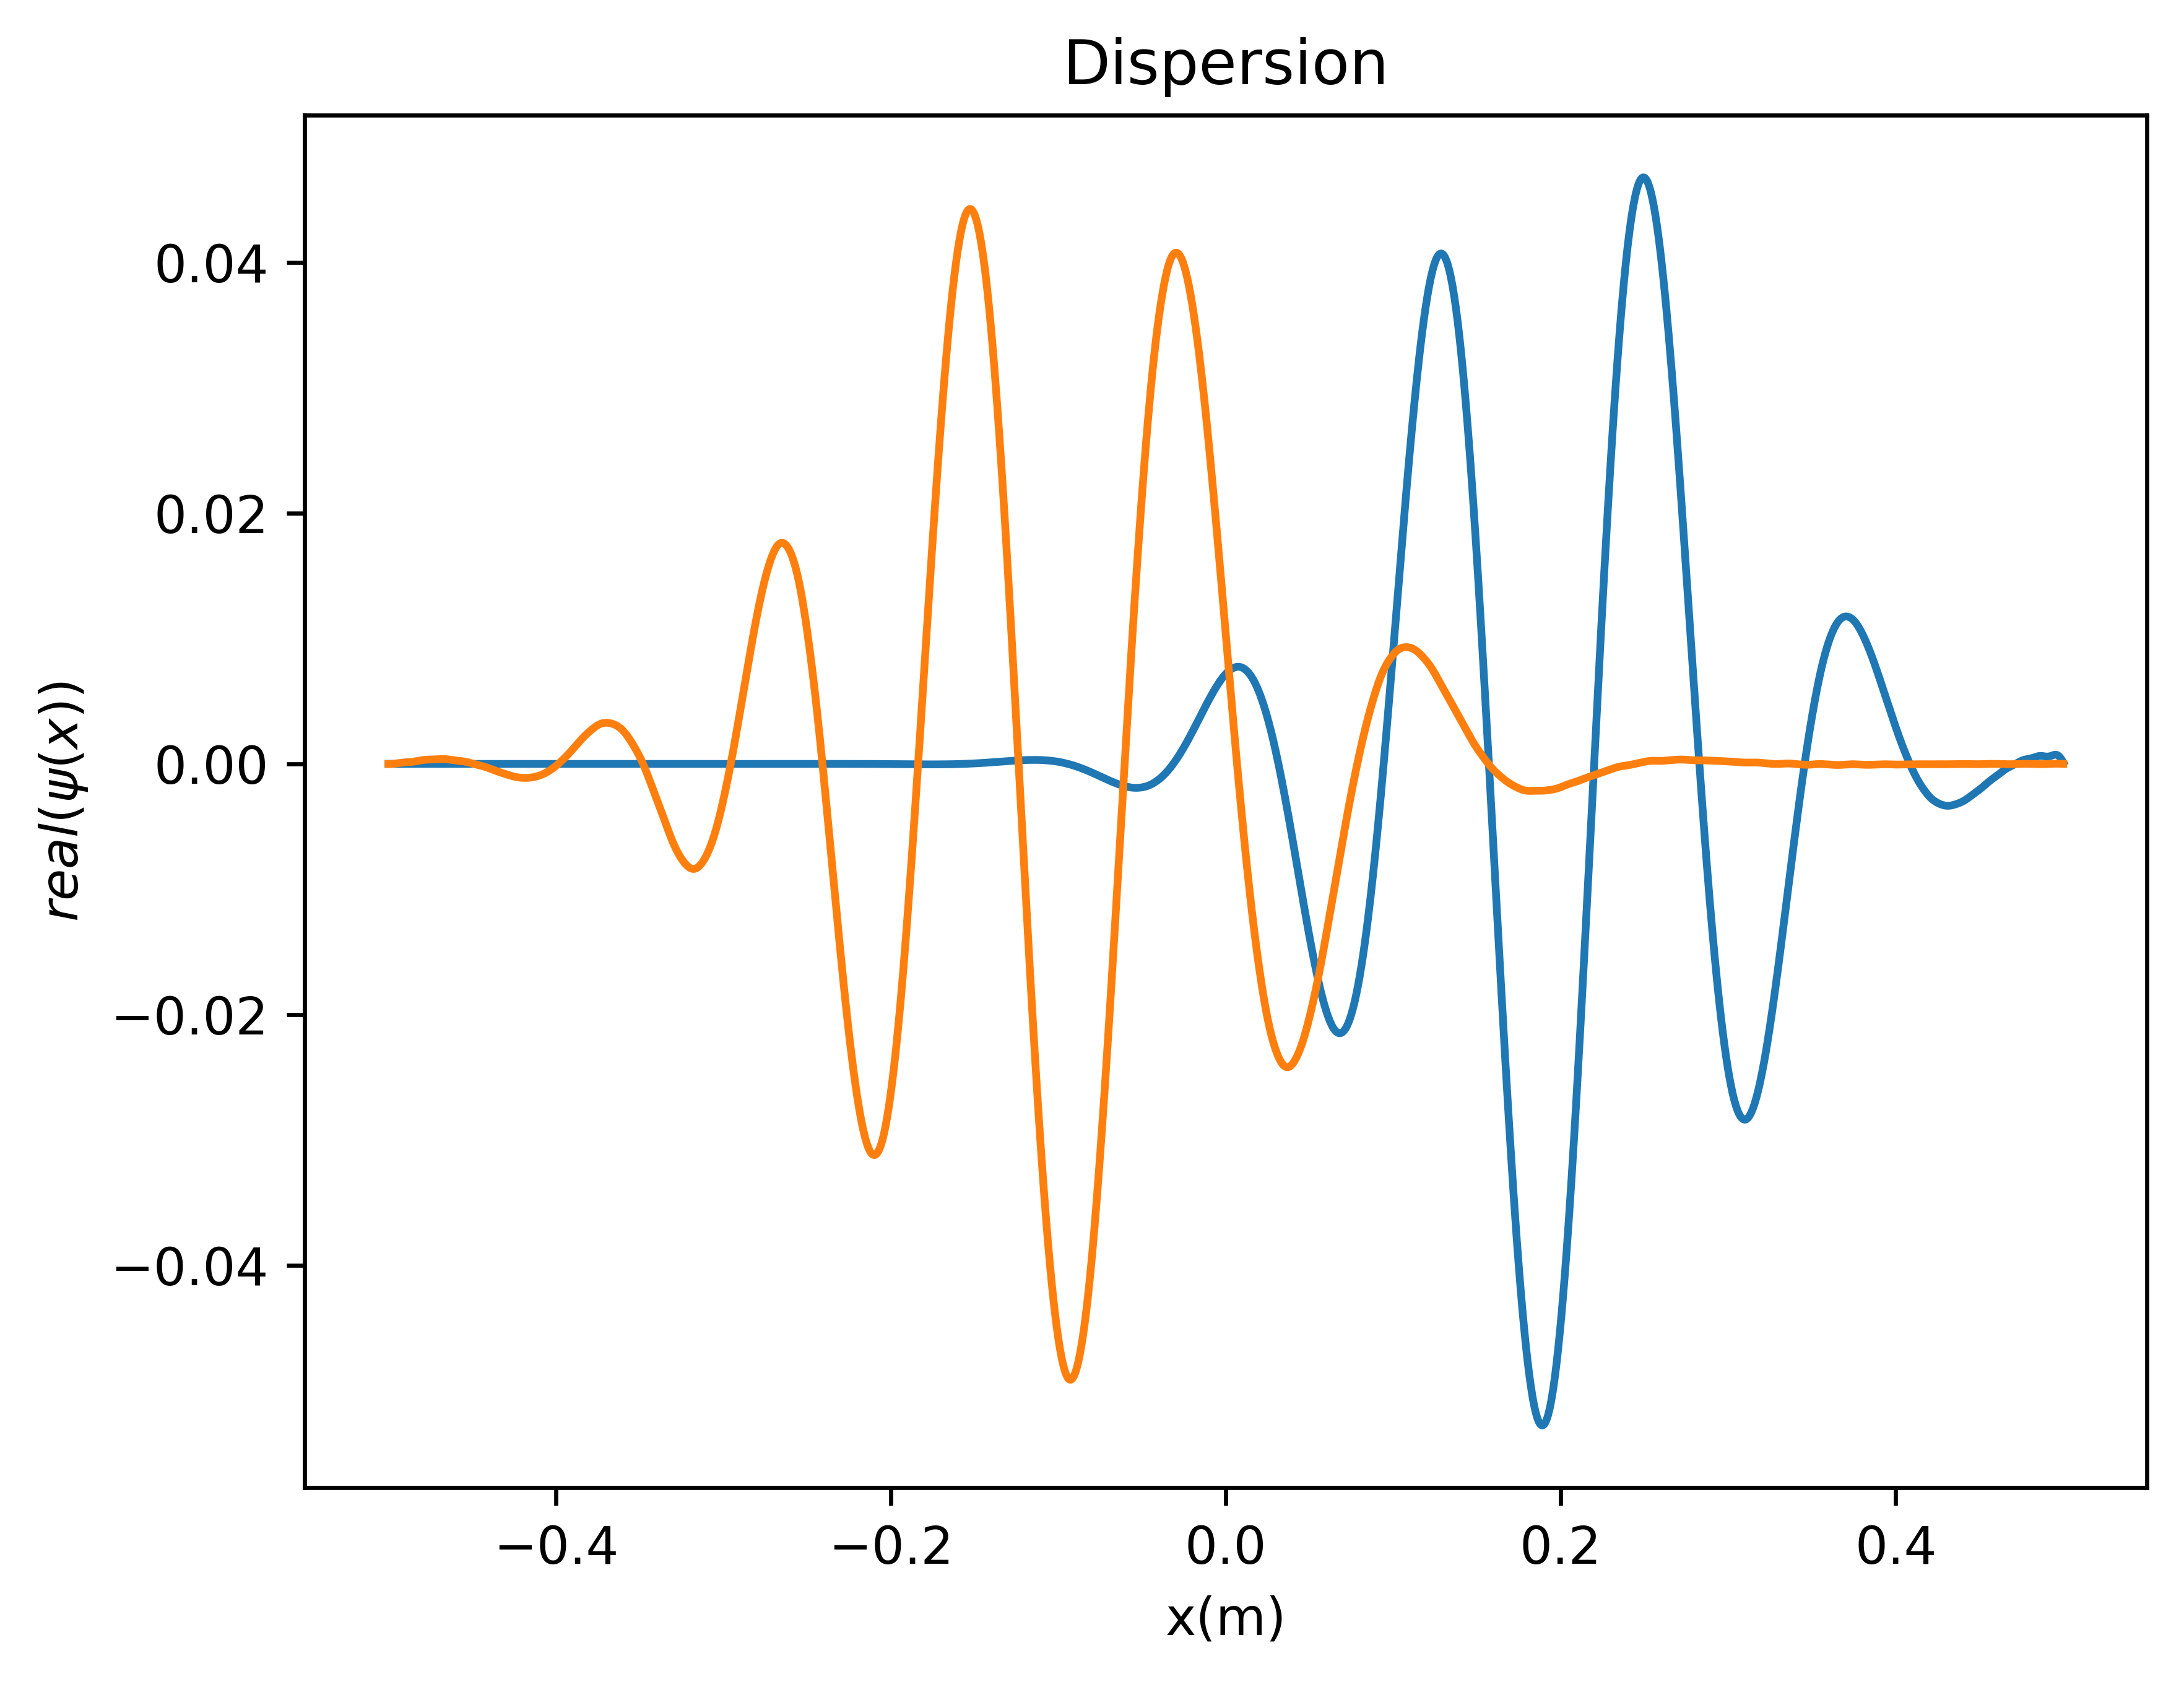
\includegraphics[scale = 0.6]{DispersionR.png}
    \caption{the real part of a wavefunction of an electron moving in as it disperse, $k = 200$, $dt = 2.5\times10^{-2}$}
    \label{fig:dispersion_realpart}
\end{figure}

\begin{figure}[H]
    \centering
    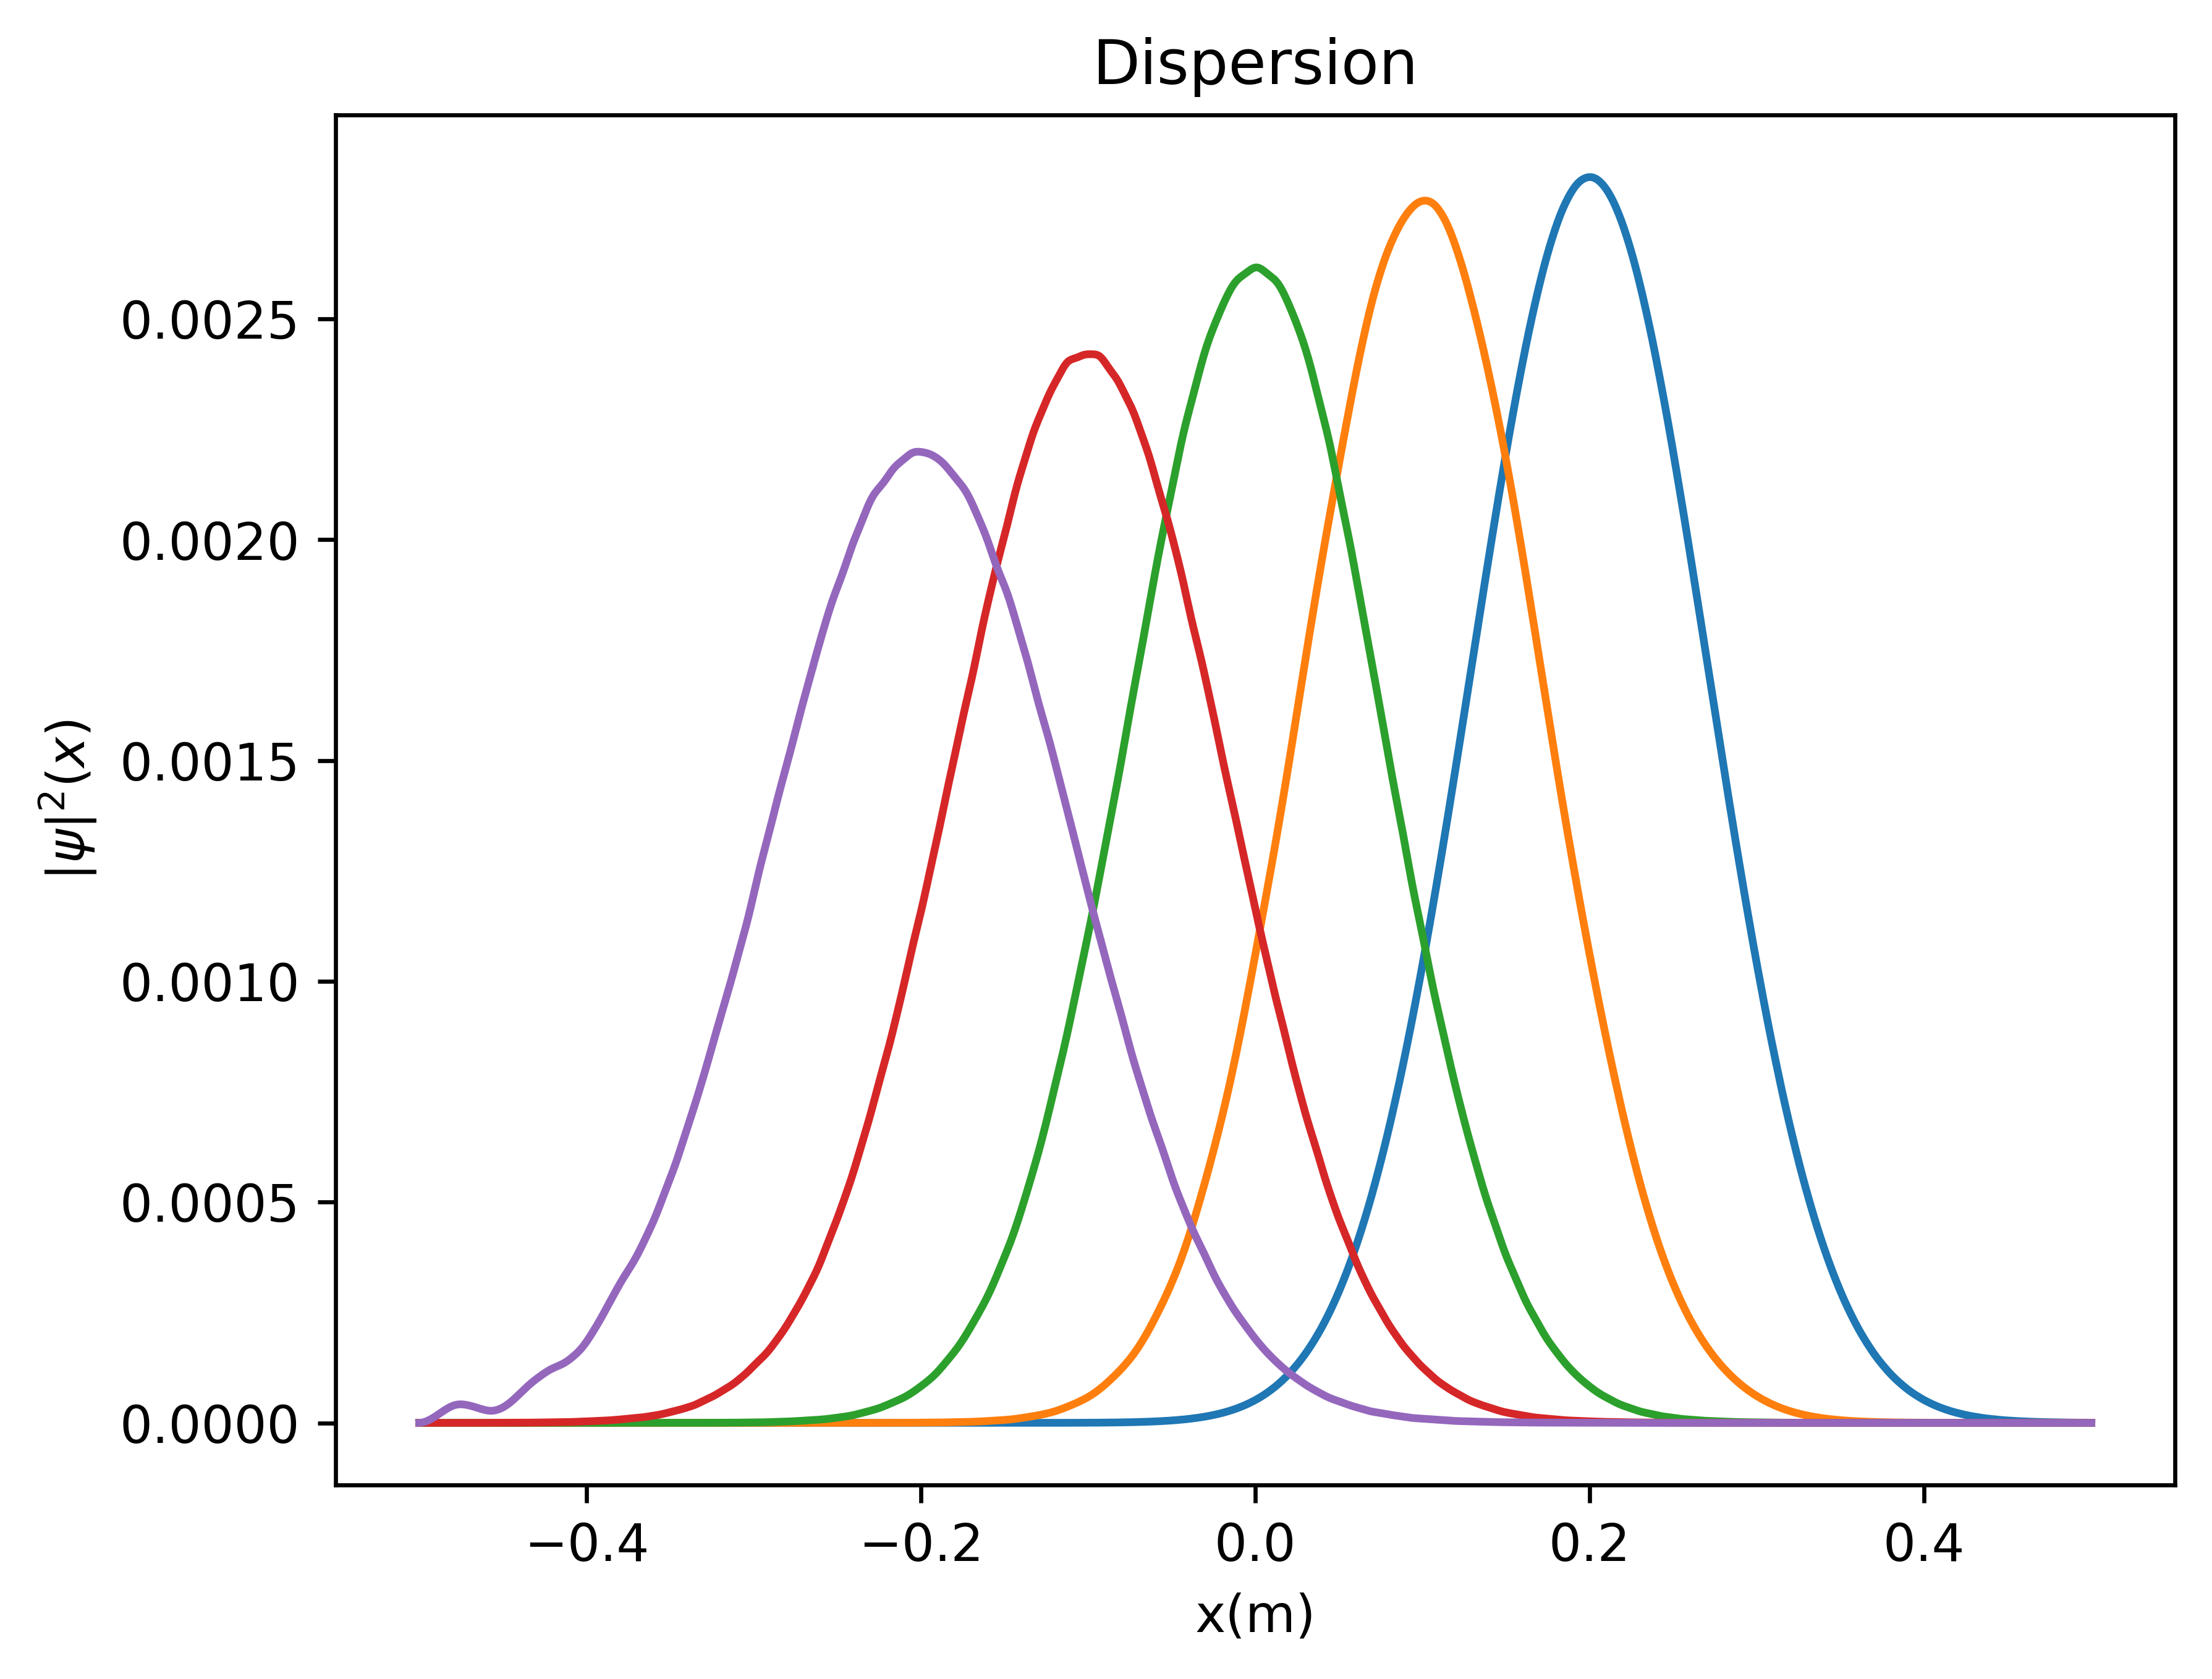
\includegraphics[scale = 0.6]{DispersionP.png}
    \caption{the probability density of an electron moving in as it disperse, $k = 200$, $dt = 5\times10^{-3}s$}
    \label{fig:dispersion_probability}
\end{figure}

\newpage

\subsection{Gaussian in an infinite well}
The following figure shows the time evolution of a gaussian initial condition:
\begin{figure}[H]
    \centering
    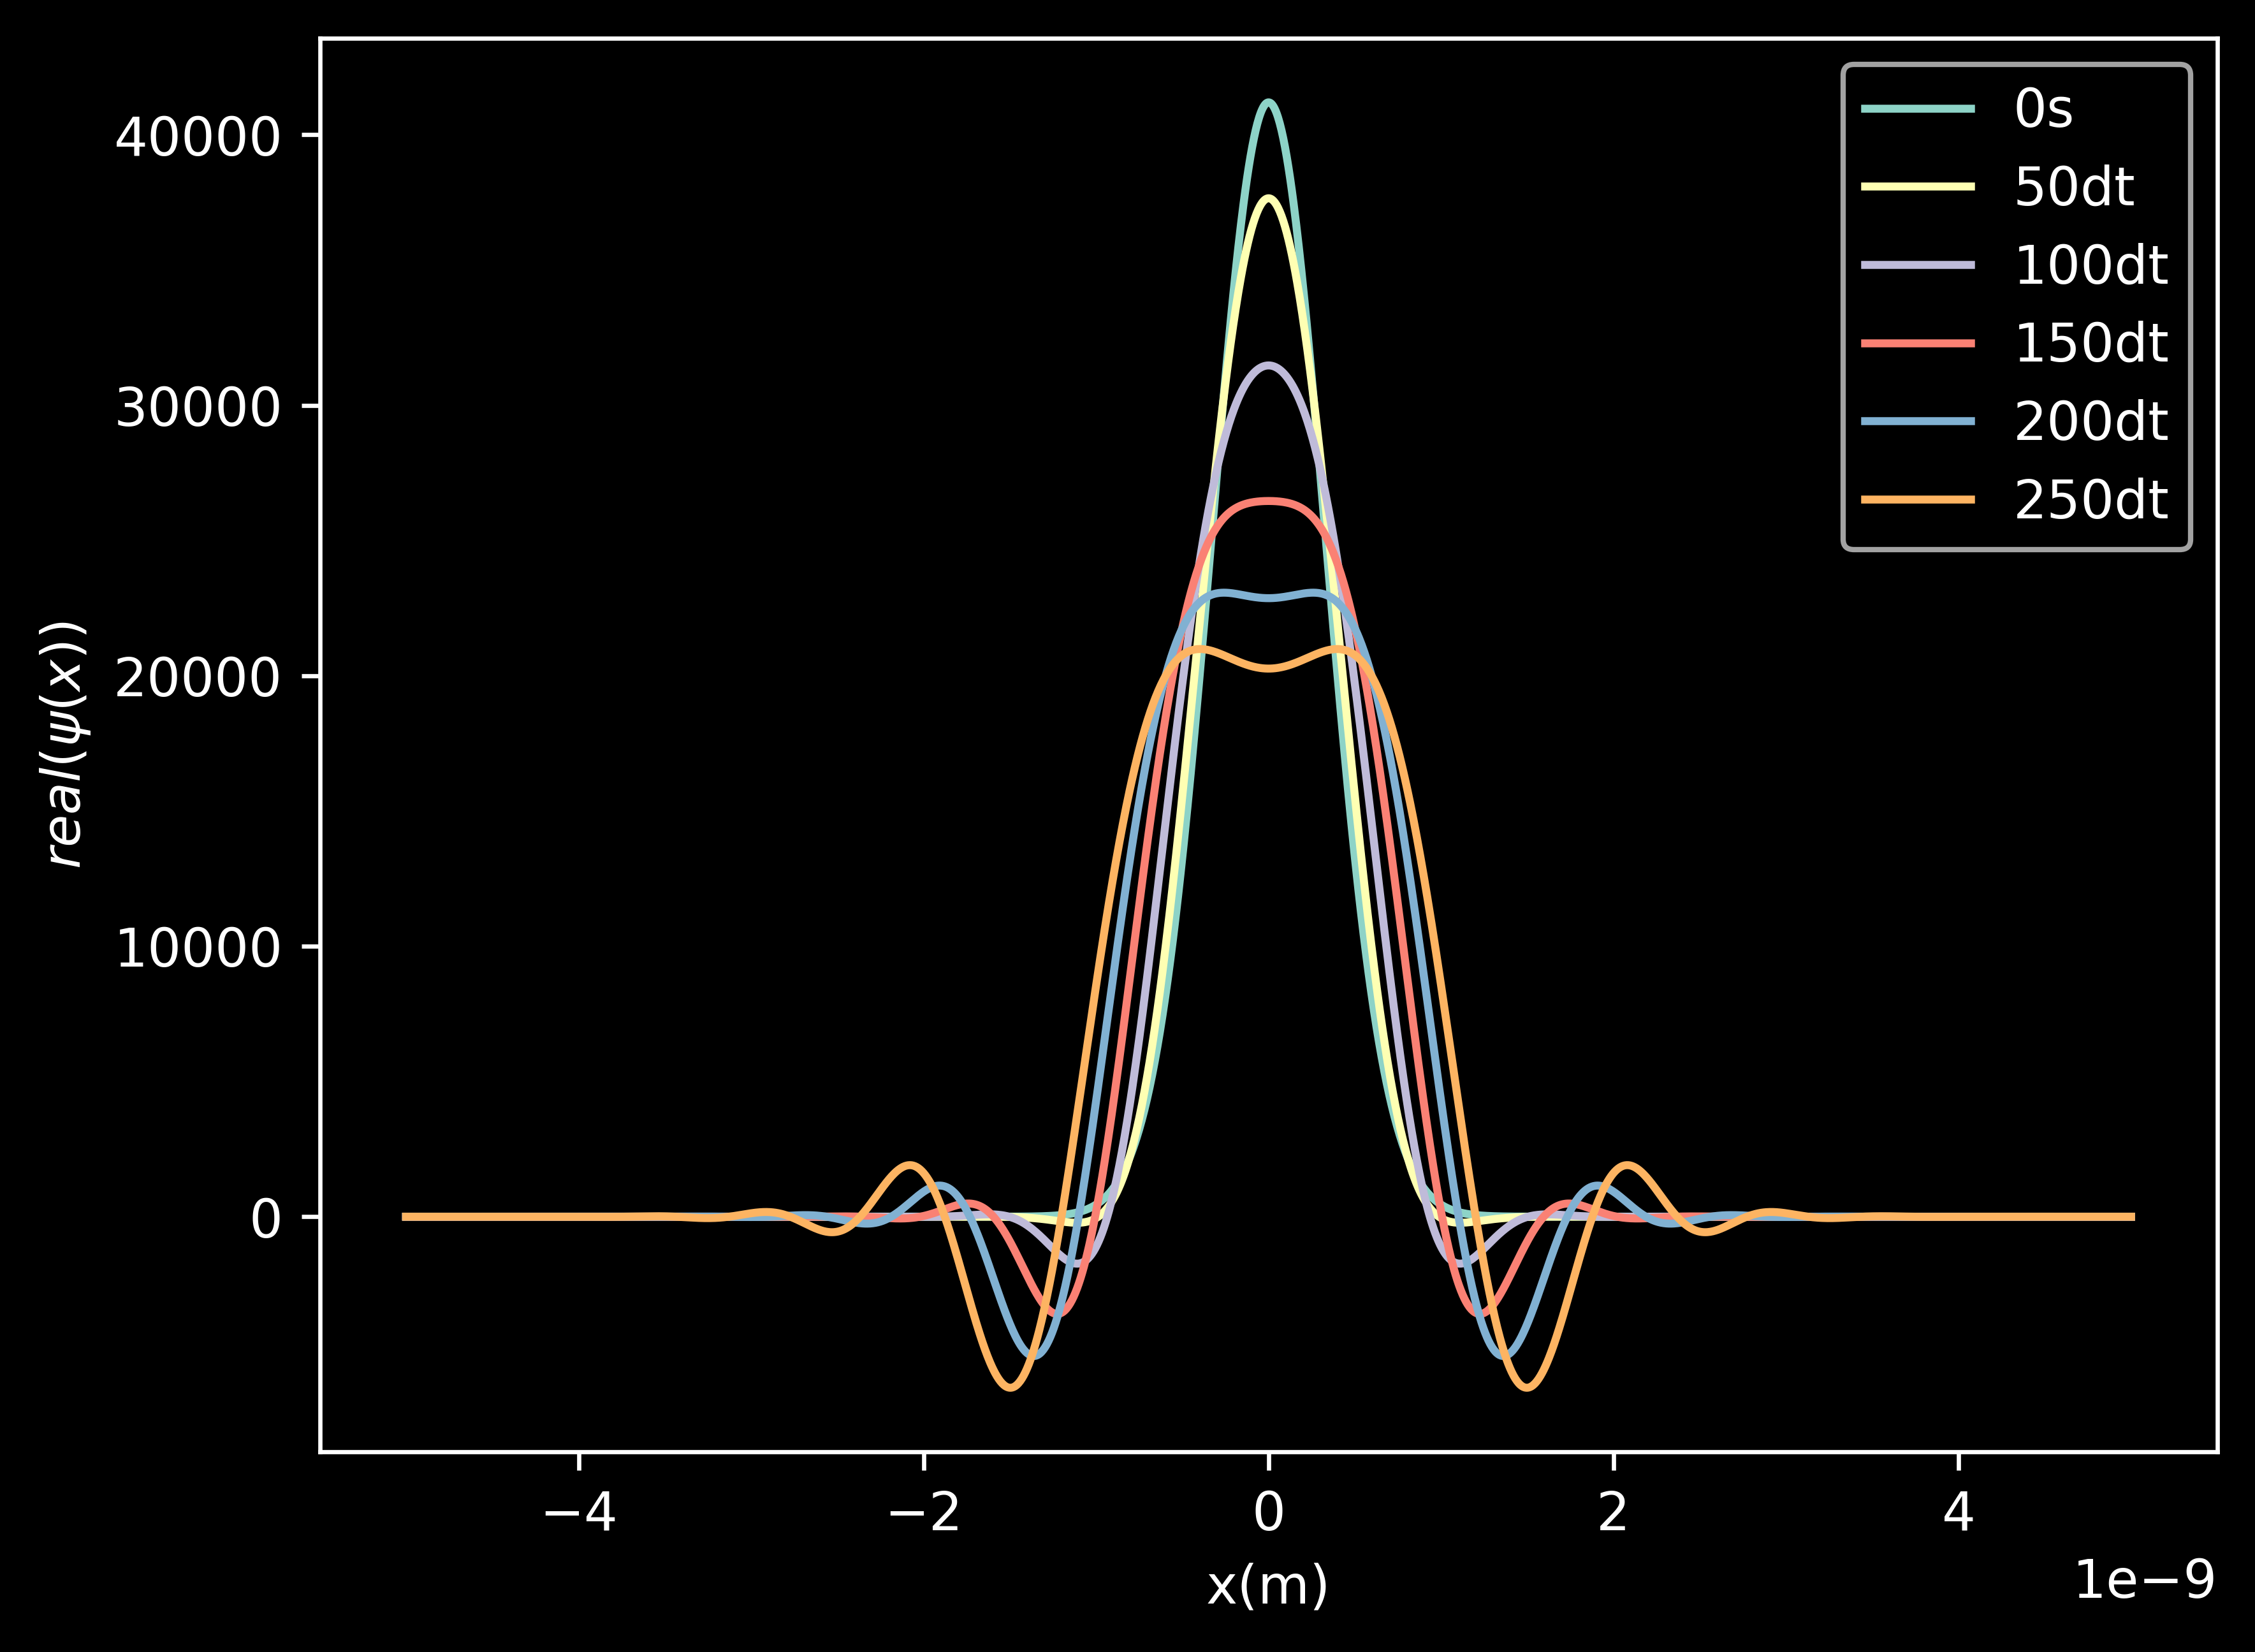
\includegraphics{dispersion.png}
    \caption{Particle in an infinite square potential well, $dt = 1\times10^{-17}$, $\sigma = \sqrt{\hbar/m_e}$.}
    \label{fig:gauss}
\end{figure}

\subsection{Tunneling}
Tunneling is an interesting quantum phenomena, assuming a potential barrier (which can be thought of as a wall), if the energy of such a barrier is bigger than the energy of the electron arriving at it, from a classical point of wiew, the electron should never be able to pass such a barrier, however, from a quantum perspective, the electron has a probability of passing through(i.e some of the wave function passes through).\\
\newpage
The probability of finding the electron after the barrier is represented by $T$.\\
\begin{table}[H]
    \centering
    \begin{tabular}{|c|c|}
    \hline
     $E/V0$& $100T$\\ \hline
    0.252& 1.51     \\ \hline
    0.977&  1.59     \\ \hline
    1.00& 21.4        \\ \hline
    1.05& 35.4         \\ \hline
    1.11& 51.1          \\ \hline
    1.21& 65.0           \\ \hline
    1.29& 74.2            \\ \hline
    1.43& 80.5             \\ \hline
    1.48& 81.3              \\ \hline
    1.54& 82.4               \\ \hline
    1.60& 83.9                \\ \hline
    1.67& 85.6                 \\ \hline
    1.74& 87.6                  \\ \hline
    1.82& 90.0                   \\ \hline
    1.91& 91.7                    \\ \hline
    2.00& 93.5                     \\ \hline
    \end{tabular}
    \caption{The percentage of electron passing through a potential barrier}
    \label{tab:my_label}
\end{table}

\begin{figure}[H]
    \centering
    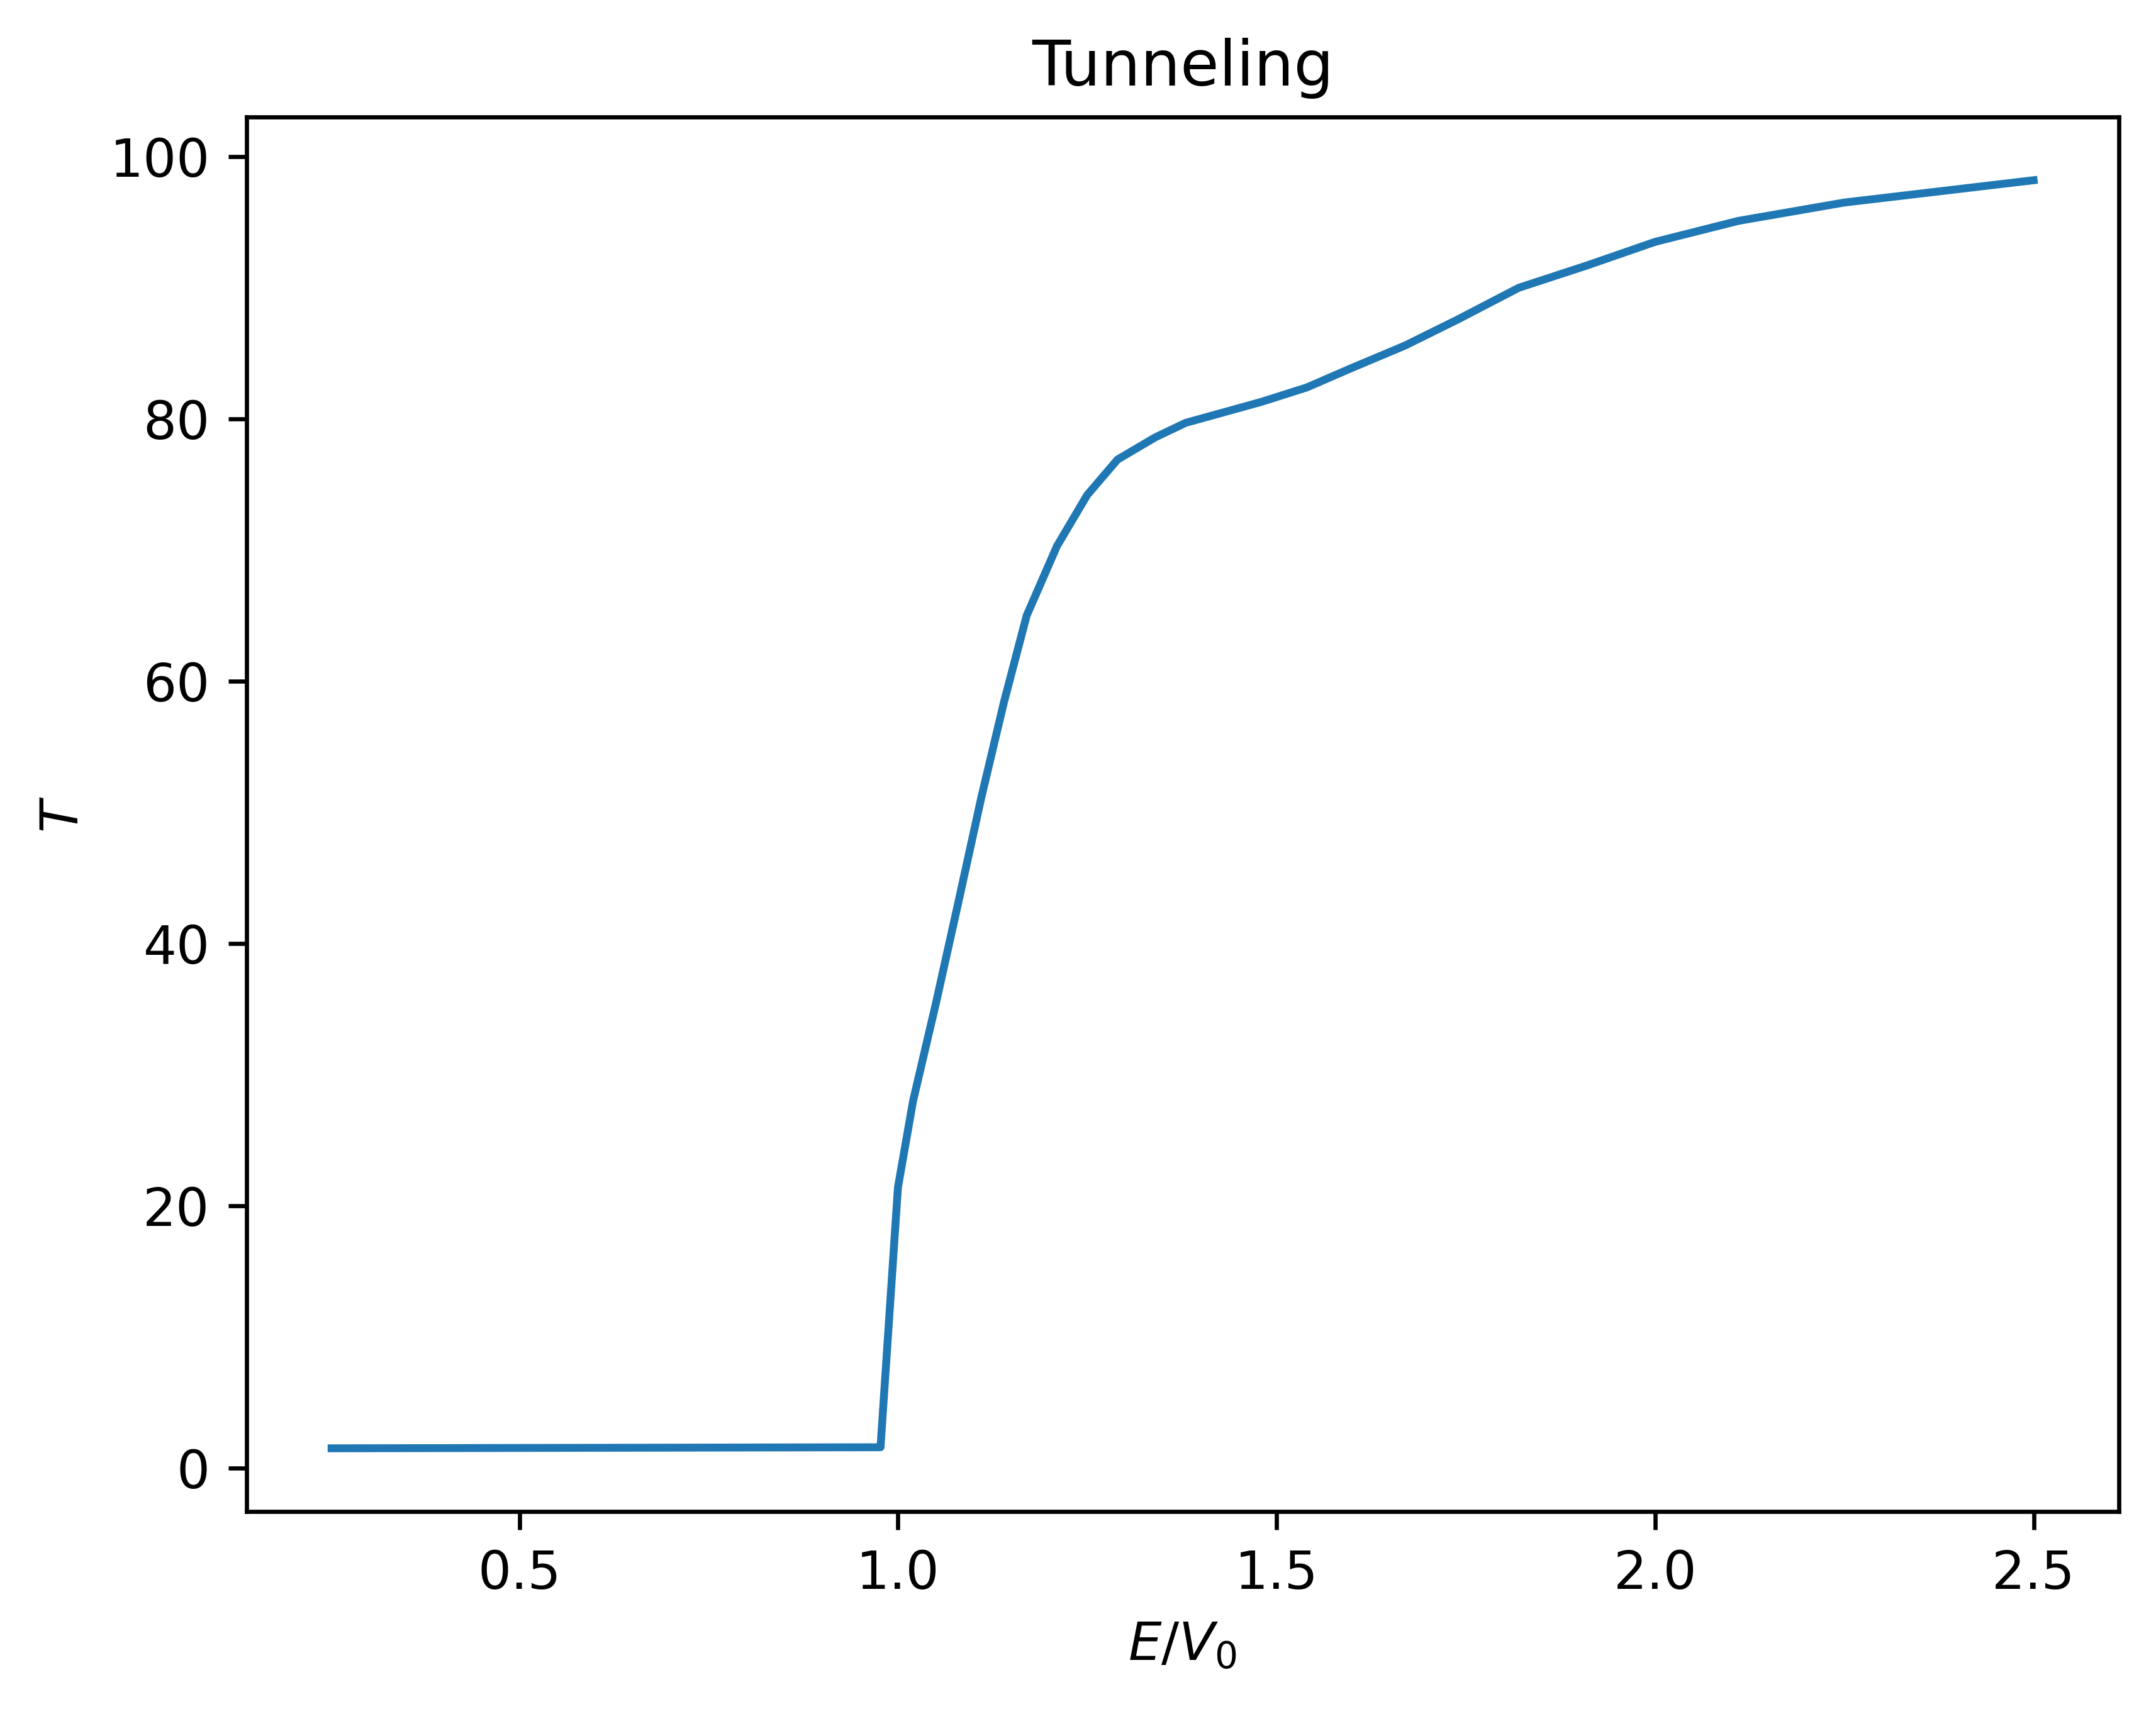
\includegraphics{tunneling.png}
    \caption{Data in Table \ref{tab:my_label}}
    \label{fig:my_label}
\end{figure}
\subsection{Double slit experiment}
Perhaps the most popular quantum mechanics experiments that depicts the wave behaviour of the electron is the double slit experiment. Even if one electron was shot towards a double slit, the electron will be diffracted, and will result is an interference pattern. In this project, the code for solving the schrodinger equation in 2 dimensions was used to simulate the double slit experiment.Bellow are 2 figures depicting the resulting solution:
\begin{figure}[H]
    \centering
    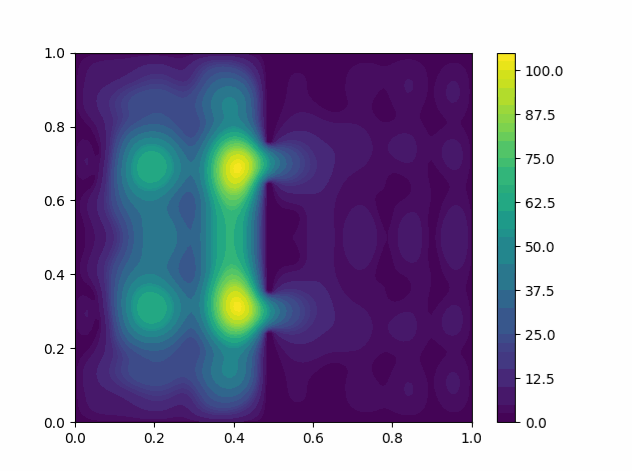
\includegraphics[scale = 0.7]{2023-02-10 (2).png}
    \caption{Double slit Experiment: one electron passing through double slit (the colour represents a value proportional to the absolute value of the wave function)}
    \label{fig:Double_Slit}
\end{figure}

\begin{figure}[H]
    \centering
    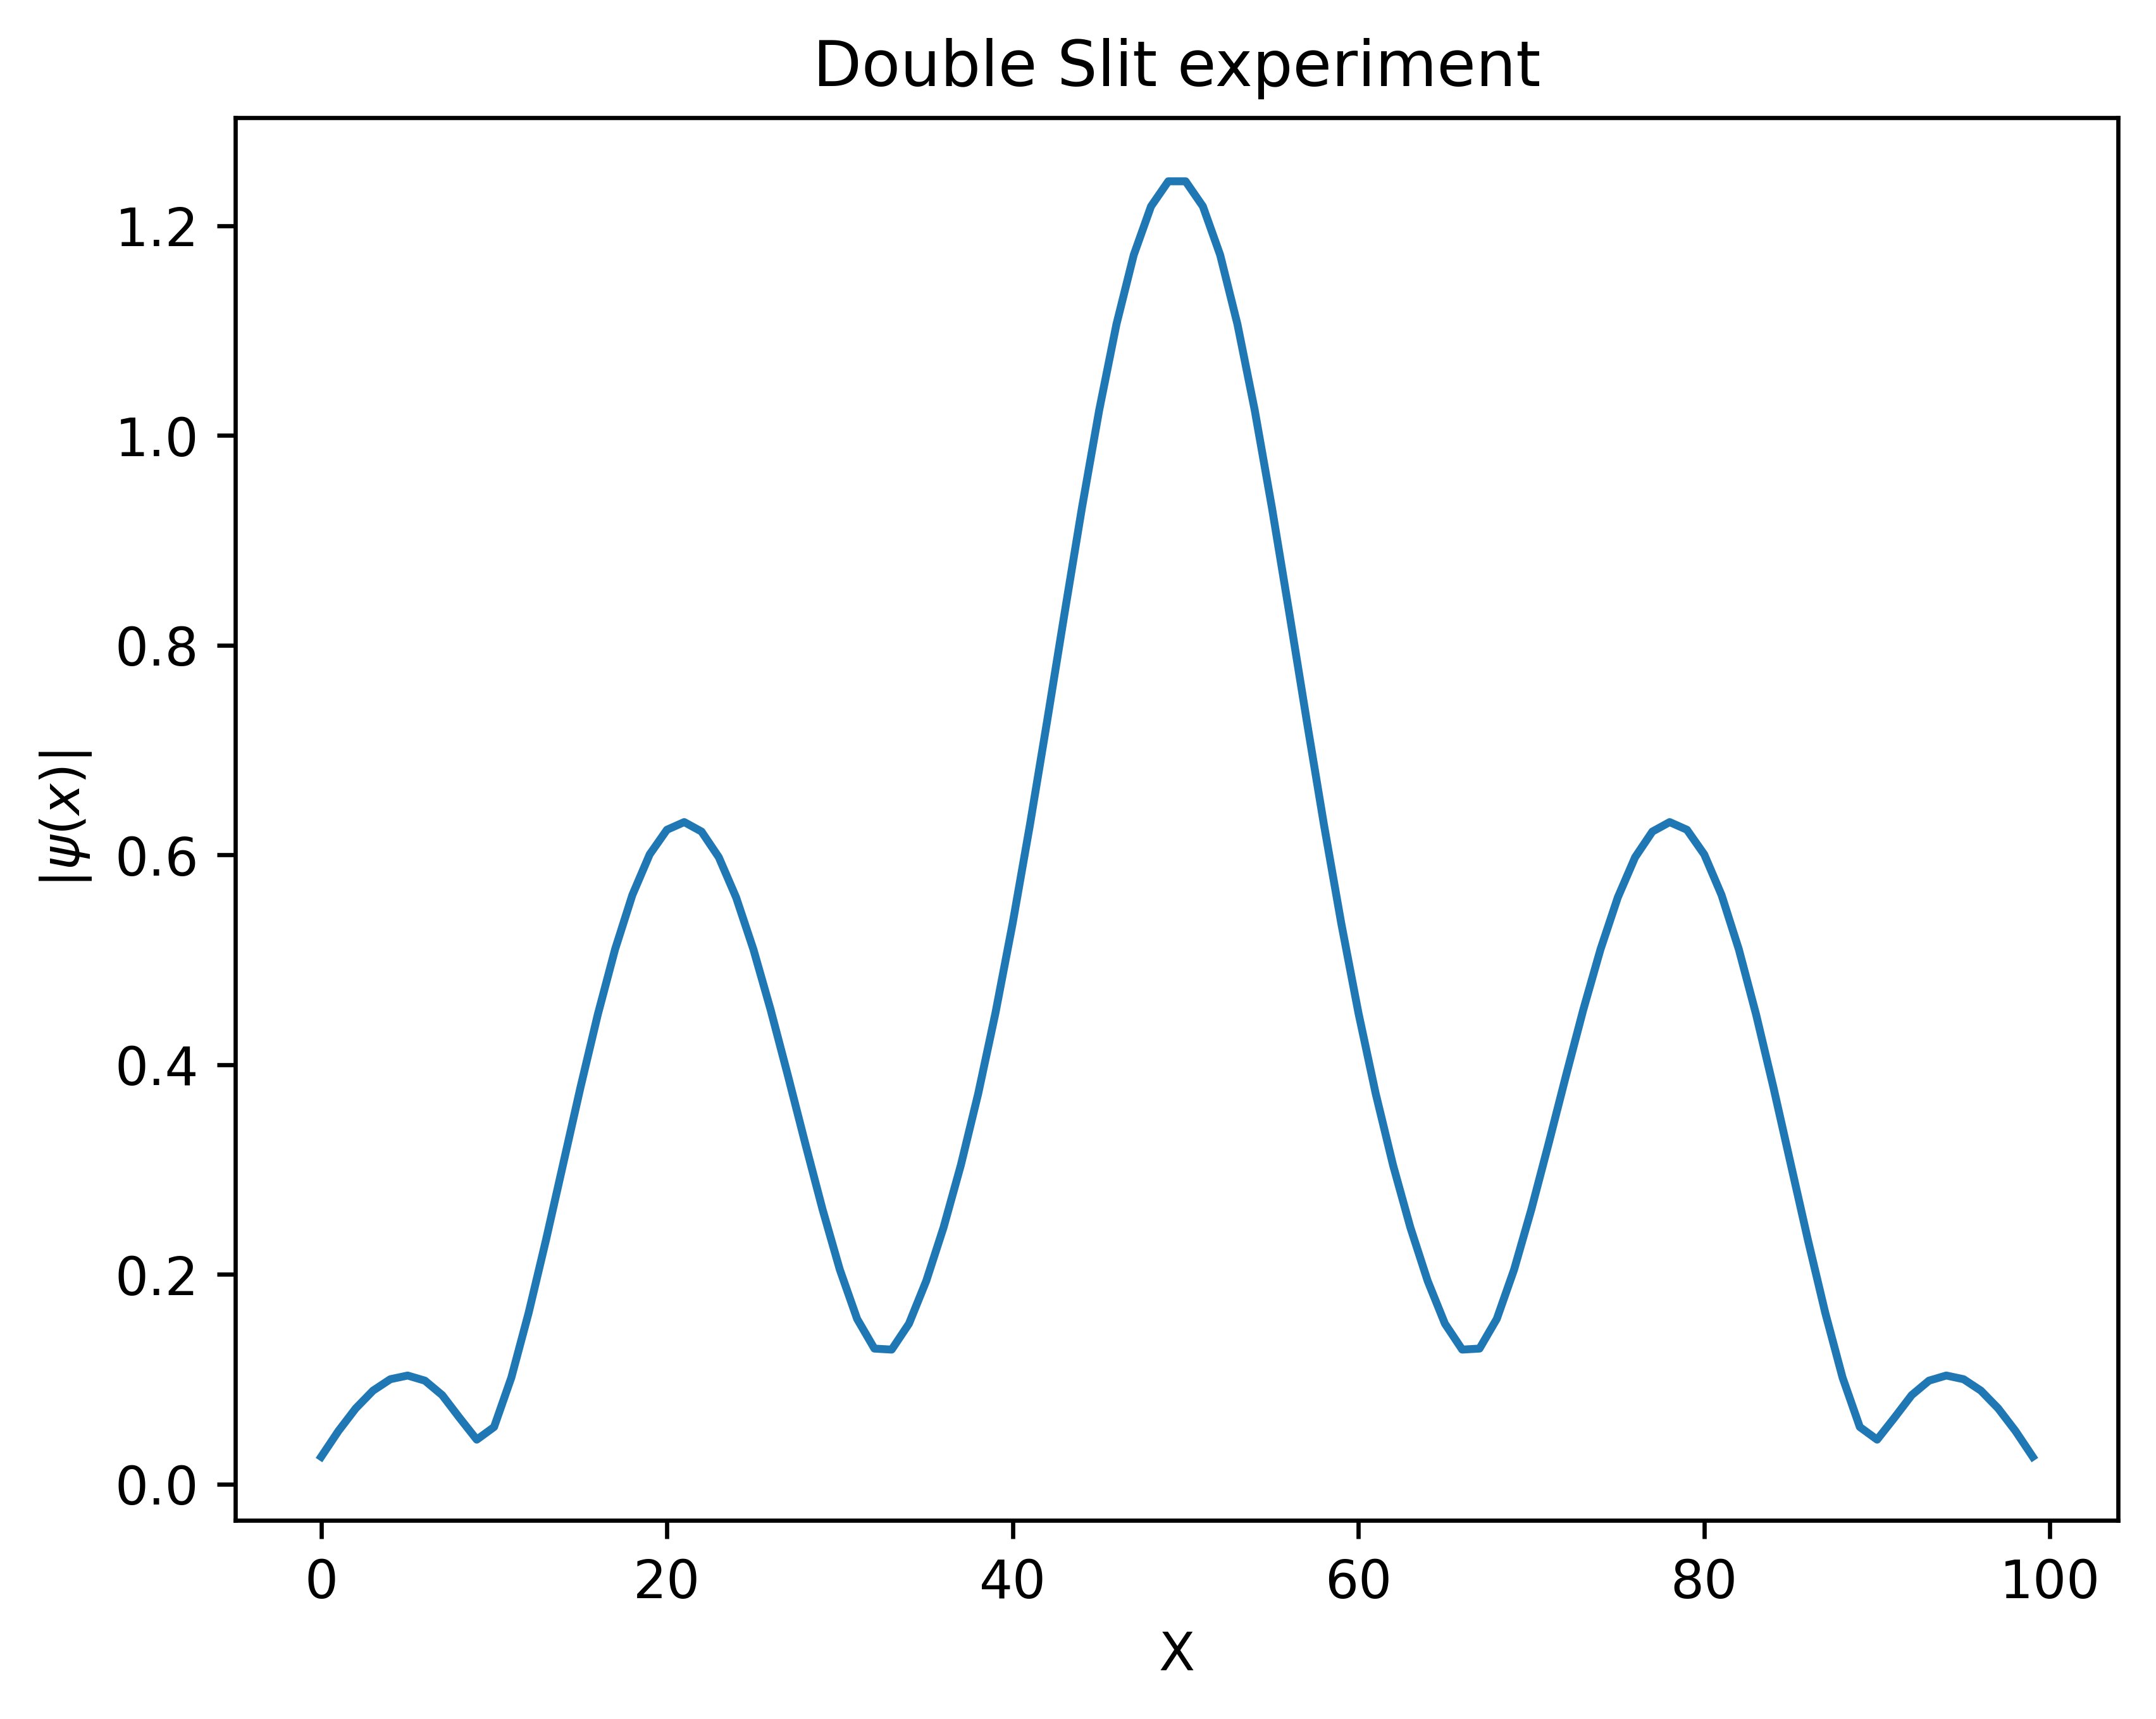
\includegraphics[scale = 0.7]{Double_slit_experiment_absolutevalue.png}
    \caption{Double slit Experiment: the resulting interference pattern}
    \label{fig:Double_Slit_2}
\end{figure}
\end{adjustwidth}


\section{\Large \textbf{Conclusion}}
\begin{adjustwidth}{1cm}{}
    Solving the Schrodinger equaiton using computational methods enables us to solve for the wave function of electron (or any quantum particle), in arbitrary potentials, and provides higher flexibility in solving it for various initial conditions, it also enable us to conduct many experiments, with lower costs than real life ones (such as the Double slit experiment).
    \subsection{Boundaries}
    All cases that were present in this project assumed the boundaries of an infinite square well, as the dimensions of such square gets bigger and bigger, electrons will behave more like an unbounded electron, or bounded by the defined potential, therefore, the 
\end{adjustwidth}


\section{\Large \textbf{References}}
\begin{adjustwidth}{1cm}{}

\begin{itemize}
    \item MIT Opencourseware Physics 8.04 lectures by Prof. Allan Adams:\url{https://www.youtube.com/watch?v=SsCeVABM4Mo&list=PLUl4u3cNGP61-9PEhRognw5vryrSEVLPr&index=13&t=2593s&ab_channel=MITOpenCourseWare}\\
    \item Wave Packets:\url{https://scholar.harvard.edu/files/schwartz/files/lecture11-wavepackets.pdf}\\
    \item Quantum Tunneling: \url{https://en.wikipedia.org/wiki/Quantum_tunnelling}
\end{itemize}
\end{adjustwidth}



\section{\Large \textbf{Appendicies}}
\subsection{The Code}
\end{document}
